%%%%%%%%%%%%%%%%%%%%%%%%%%%%%%%%%%%%%%%%
%% MCM/ICM LaTeX Template %%
%% 2022 MCM/ICM           %%
%%%%%%%%%%%%%%%%%%%%%%%%%%%%%%%%%%%%%%%%
\documentclass[12pt]{article}
\usepackage{geometry}
\setlength\headheight{24pt}
\geometry{left=1in,right=0.75in,top=1in,bottom=1in}
\usepackage[utf8]{inputenc}
%%%%%%%%%%%%%%%%%%%%%%%%%%%%%%%%%%%%%%%%
% Replace ABCDEF in the next line with your chosen problem
% and replace 1111111 with your Team Control Number
\newcommand{\Problem}{E}
\newcommand{\Team}{2200973}
%%%%%%%%%%%%%%%%%%%%%%%%%%%%%%%%%%%%%%%%

\usepackage{newtxtext}
\usepackage{amsmath,amssymb,amsthm}
\usepackage{newtxmath} % must come after amsXXX
%\usepackage[pdftex]{graphicx}
\usepackage[table]{xcolor}
\usepackage{fancyhdr}

%%%%%%%%%%%%%%%%%个人添加的导言区,使用xelatex进行编译
\usepackage{graphicx} %去掉了pdftex的选项,官方summary sheet带有此选项
\usepackage{lastpage} %用于读取最后一页,更改了页眉变为 x of lastpage
\usepackage{indentfirst} %配置章节标题命令之后的第一段缩进
\usepackage{booktabs} %科技论文的三线段表宏包支持,上下线段建议设置为1.5pt
\usepackage{array,tabularx} %表格扩展功能宏包
\usepackage[hidelinks]{hyperref} %目录超链接
\usepackage{pythonhighlight} %python代码支持
\usepackage[style=ieee]{biblatex} %参考文献格式
\usepackage{colortbl}
\addbibresource{reference.bib}
%%%%%%%%%%%%%%%%%

\lhead{\textsf{Team \# \Team}}
\rhead{}
\cfoot{}

\newtheorem{theorem}{Theorem}
\newtheorem{corollary}[theorem]{Corollary}
\newtheorem{lemma}[theorem]{Lemma}
\newtheorem{definition}{Definition}

%%%%%%%%%%%%%%%%%%%%%%%%%%%%%%%%
\begin{document}
\graphicspath{{graph/}}  % Place your graphic files in the same directory as your main document
\DeclareGraphicsExtensions{.pdf, .jpg, .tif, .png}
\thispagestyle{empty}
\vspace*{-16ex}
\centerline{\begin{tabular}{*3{c}}
        \parbox[t]{0.3\linewidth}{\begin{center}\textbf{Problem Chosen}\\ \Large \textcolor{red}{\Problem}\end{center}}
         & \parbox[t]{0.3\linewidth}{\begin{center}\textbf{2022\\ MCM/ICM\\ Summary Sheet}\end{center}}
         & \parbox[t]{0.3\linewidth}{\begin{center}\textbf{Team Control Number}\\ \Large \textcolor{red}{\Team}\end{center}} \\
        \hline
    \end{tabular}}
%%%%%%%%%%% Begin Summary %%%%%%%%%%%
% Enter your summary here replacing the (red) text
% Replace the text from here ...
{\centering\section*{The Optimal Strategies of Forest Management}}
{\centering\subsection*{Summary Sheet}}
{\large 	Forest is the largest carbon pool in the terrestrial ecosystem, which plays a very important and unique role
    in reducing the concentration of greenhouse gases in the atmosphere and slowing down global warming.
    The expansion of forest cover is an important mitigation measure that is economically feasible and less costly in the future.
    To study the carbon sequestration capacity of forests and its economic value,
    we established two models: Model I, the best carbon sequestration rate model based on the Logistic Growth Model and BEF;
    Model II is the best economic benefit model based on the Logistic Growth Model.

    In Model I, we solve the problem of how to predict the future amount of carbon
    sequestration in forests and their products. To predict the amount of carbon
    sequestration in the forest, we first predict the future growth and development
    of the forest according to the Logistic Growth Model and obtain the change
    curve of the number of timber trees in the forest with time. And then calculate
    that specific stand volume of the forest in combination with the species of the
    tree which is in the forest. Then we calculate the total biomass in the forest
    according to the BEF of different forests and calculate the specific carbon
    content in the forest. According to the curve of forest carbon sequestration
    over time, we obtained the forest size under the maximum carbon sequestration
    rate.

    In Model II, we solve the problem of how to determine the best time and amount
    of logging in the case of considering economic benefits. After considering many
    factors such as inflation coefficient, logger's salary, logging efficiency,
    timber market unit price, and so on, we calculate the best logging time and the
    best number of loggers according to the Logistic growth model and the method of
    differential equation. We obtained the forest size under the best economic
    benefit of the forest was determined.

    In addition, we also predict the carbon sequestration of forests after 100
    years and propose the best strategy for cutting down trees. And wrote a news
    report to educate the public about forest management.}

\begin{table}[b]%%%关键词区域,放在浮动体中了
    \noindent\textbf{Keywords:} BEF\cite{Fang};Differential Equation;Logistic Growth Model
\end{table}
% to here
%%%%%%%%%%% End Summary %%%%%%%%%%%
\setcounter{page}{1} %%%重设计数器,从第一页开始
%%%%%%%%%%%%%%%%%%%%%%%%%%%%%%
\clearpage
\pagestyle{fancy}
% Uncomment the next line to generate a Table of Contents
\rhead{\textsf{Page \thepage\ of \pageref{LastPage}}}
\tableofcontents
\newpage
%\setcounter{page}{1}
%\rhead{Page \thepage\ of \pageref{LastPage}}
%%%%%%%%%%%%%%%%%%%%%%%%%%%%%%
%Begin your paper here\cite{YiZhao-481}
\section{Introduction}
\subsection{Problem Background}
Carbon sequestration plays an important role in improving the current human
living environment. To mitigate the effects of climate change, we need to take
action to reduce the content of greenhouse gases such as carbon dioxide in the
atmosphere. Forest carbon sequestration is the most economical and
environmental protection way at present.

Thanks for the gift of nature! At present, there are still large areas of
natural forests on earth to help us absorb carbon dioxide and produce oxygen.
Unfortunately, with the continuous improvement of the human industrial level,
the existing forest carbon sequestration capacity is worrying. We must and have
to plant trees artificially. Because of its unique ecological, scientific, and
economic values, we do not recommend cutting down or destructive management of
natural forests. Plantation has many factors, such as single tree species, high
value of forest products, easy management, and so on, which can be reasonably
cut down or planted under certain conditions. Therefore, in this paper, we
mainly discuss plantations. All the time starting points in the article are the
completion points of the plantation.
\subsection{Restatement of the Problem}
Considering the background information and restricted conditions identified in
the problem statement, the following problems are needed to be solved:
\begin{description}
    \item[\ddag{} Problem 1] Develop a carbon sequestration model to determine how much%
        carbon dioxide a forest and its products can be expected to sequester over time.
    \item[\ddag{} Problem 2] Forest management strategies considering economic benefits.
    \item[\ddag{} Problem 3] What kind of trees will be cut down.
    \item[\ddag{} Problem 4] How much carbon dioxide will this forest and its products sequester over 100 years.
\end{description}
\subsection{Our Work}
In Model I, we build a model to simulate the growth process of a tree and the
relationship between trees and total carbon sequestration in the forest. We
mainly use the logistic growth prevention model and learn from the BEF factor
method to lay a good foundation for the establishment and evaluation of the
later model and the proposal of Solutions.

In Model II, we mainly consider the economic value of forests, build a
mathematical model from the timing and quantity of deforestation, accurately
calculate the optimal timing and quantity of deforestation, and simulate the
economic benefits that forests can obtain under this condition. At this time,
we noticed that we only determined the number of felling, so we constructed
different mathematical models to discuss which trees should be felled and which
trees should be retained, and gave specific practical schemes.

In the next part(\ref{611}), we calculate how much carbon dioxide forests and
forest products will absorb in 100 years in our plan. At the same time, we also
give reasonable strategies to transition the forest management plan from the
existing schedule to the new schedule.

At the end of our articles, we wrote a non-technical newspaper article, which
roughly described our research ideas and research results, and explained the
truth to the public and the local community in a pertinent tone, so that the
local community can approve and adopt our plan.
\begin{figure}[htb]
    \centering
    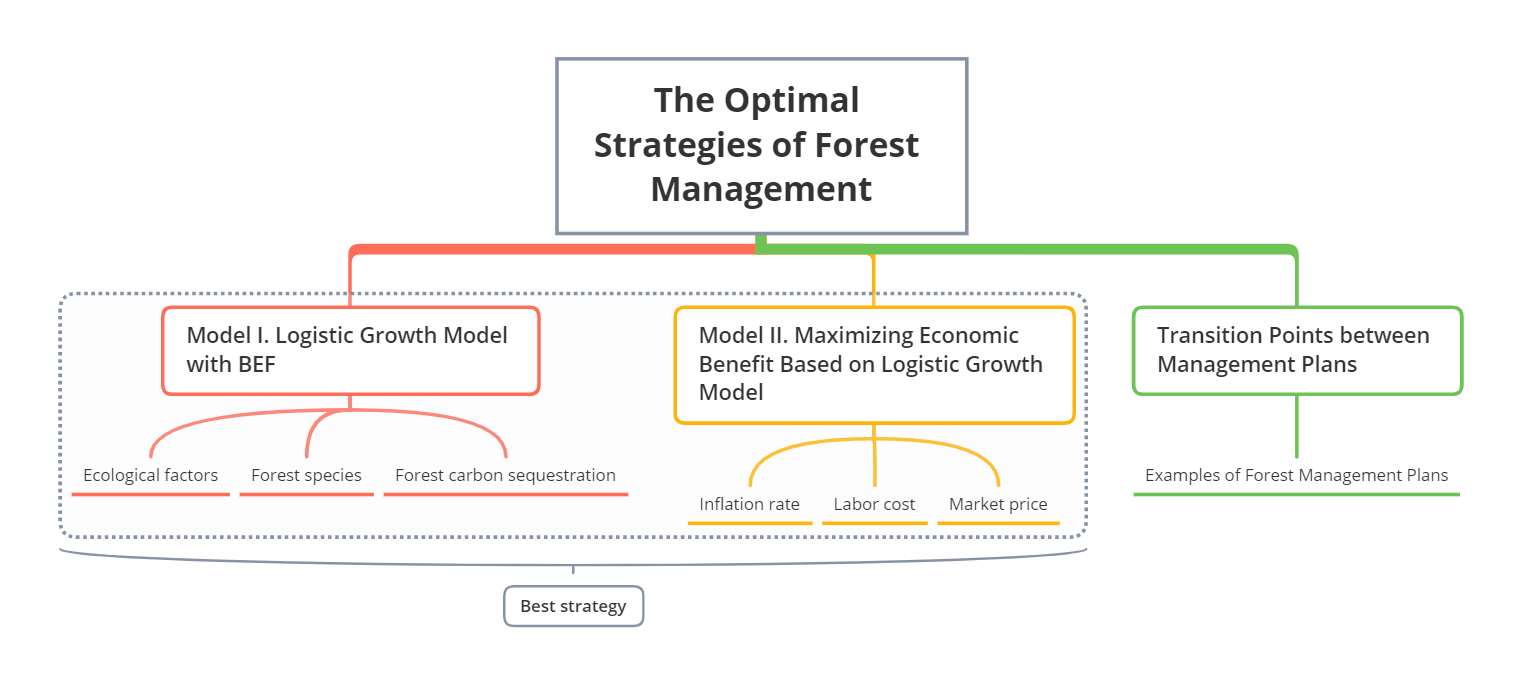
\includegraphics[width=17cm]{xmind.png}
    \caption{The Structure of Our Paper}
\end{figure}

\section{Assumptions, Justifications and Reasons}
\begin{description}
    \item[\dag Assumption 1:]We assume that the stand biomass in the forest is only provided by mature trees.\\
    \textbf{Justification:}{ }The young trees are small in volume and carbon sequestration, and contribute less to stand biomass;
    Over mature trees are vulnerable to death or collapse from a variety of causes. Therefore,
    it is reasonable to think that the stand biomass in the forest is only provided by mate trees.
    \item[\dag Assumption 2:]We assume that all forests develop normally without biological invasion and natural disasters.\\
    \textbf{Reason:}{ }Biological invasion and natural disasters will greatly change the state of forests, which are difficult to predict.
    \item[\dag Assumption 3:]We assume that there is no forest desertification or negative growth caused by human factors.\\
    \textbf{Reason:}{ }Human activities are difficult to predict.
\end{description}

\section{Notations and Definitions}
\subsection{Notations}
The key mathematical notations used in this paper are listed in Table
\ref{table1}.
\begin{table}[ht]
    \caption{Notations Used in This Paper}\label{table1}
    \begin{tabularx}{\textwidth}{>{\centering\arraybackslash}X>{\centering\arraybackslash}p{14cm}}
        \toprule
        \textbf{Symbol} & \textbf{Description}                                                     \\
        \midrule
        $t$             & Time elapsed since the forest was formed                                 \\
        \midrule
        $x(t)$          & Variation function of the number of mature trees per unit area with time \\
        \midrule
        $x_m$           & Maximum number of mature trees per unit area                             \\
        \midrule
        $r$             & Innate rate of increase
        \footnotemark[1]
        \footnotemark[2]                                                                           \\
        \midrule
        $x_0$           & Initial number of wood                                                   \\
        \midrule
        $V_a$           & Volume of a single mature tree                                           \\
        \midrule
        $C_a$           & Carbon sequestration                                                     \\
        \midrule
        $C_a'$          & Carbon fixation rate                                                     \\
        \midrule
        $S$             & Acreage of forest                                                        \\
        \bottomrule
    \end{tabularx}

\end{table}\\
\footnotetext[1]{This value is affected by many factors, such as the location of the forest, light, precipitation, temperature and so on. Or call it as \emph{environmental factors.}}
\footnotetext[2]{this is an example of a footnote.}
\subsection{Definitions}
\noindent\emph{BEF:}
\begin{quote}
    Defined as the ratio of all stand biomass to growing stock volume.\cite{Fang}
\end{quote}
\emph{Mature trees}
\begin{quote}
    Mature trees can be made into various products.
    Usually, we cut down mature trees and over mature trees.
\end{quote}

\section{Model I. Logistic Growth Model with BEF}
To determine the best forest management model to achieve the best carbon
sequestration effect, we carried out the following work.
\begin{figure}[htb]
    \centering
    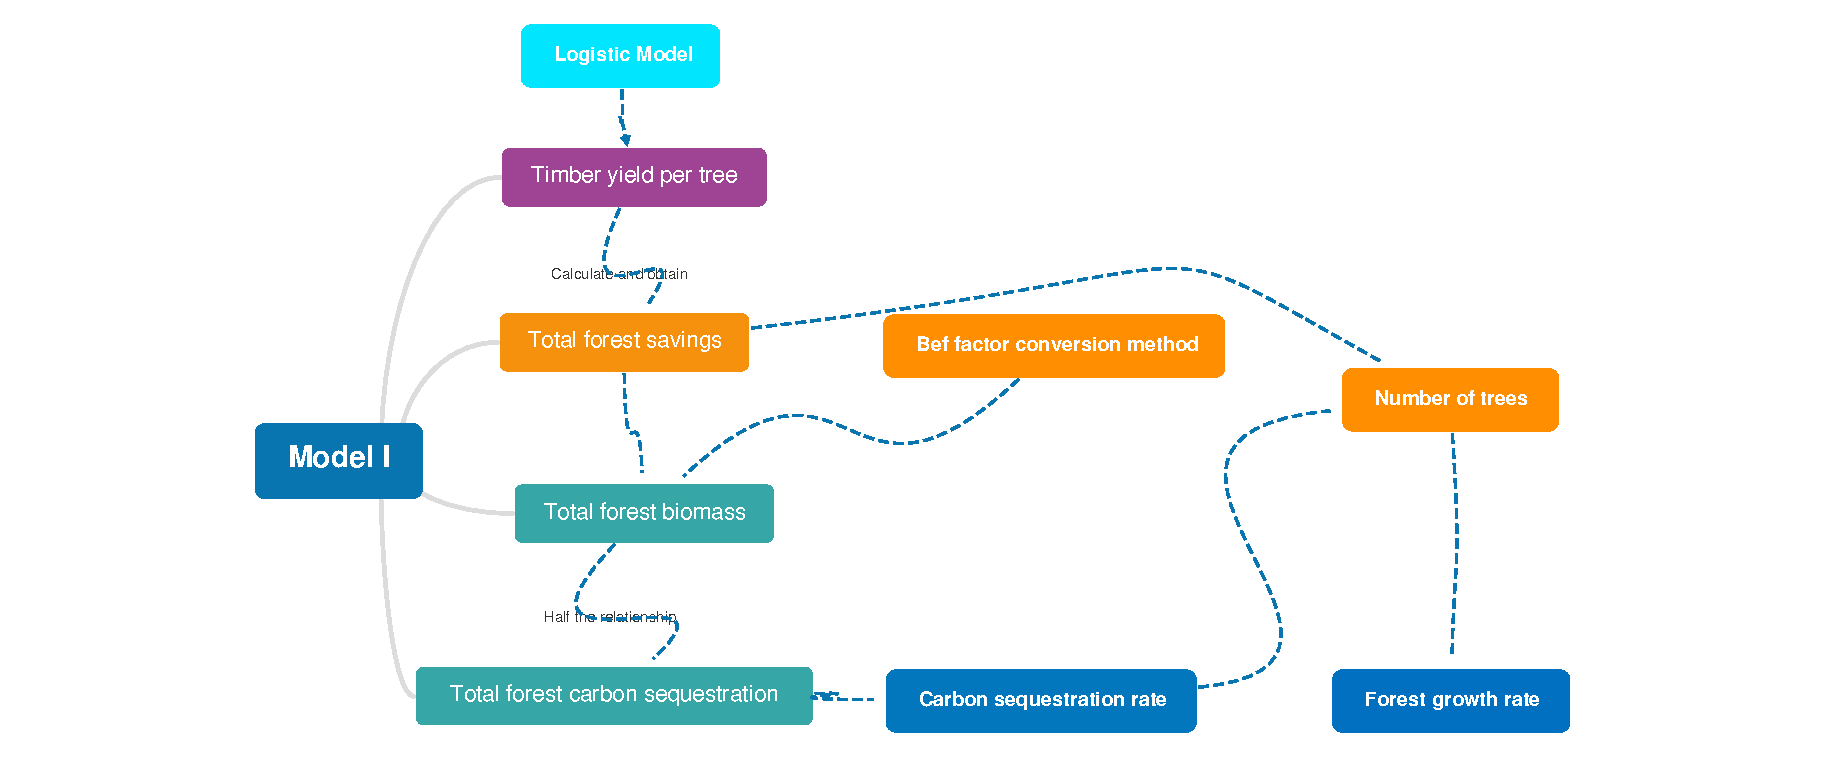
\includegraphics[width=18cm]{Model I.pdf}
    \caption{Mind map of Model I}
\end{figure}
\subsection{Differential Equation Modeling}
In the real environment, it can be known from the basic knowledge of biology
that the population presents a logistic growth pattern under the condition of
limited resources. The trees in the forest constitute the basic population, the
tree growth space is limited, and the total amount of inorganic salts is
limited. Therefore, the growth in the number of mature trees conforms to the
logistic growth model\cite{F2,2009Ecology}.

According to the Logistic Growth Model, we can get the following equation:
\begin{align}
    \left\{
    \begin{array}{l}
        x^\prime\left(t\right)=rx\left(1-\dfrac{x}{x_m}\right) \\
        x(0)=x_0
    \end{array} \right.
    \label{logistic}
\end{align}
Integrating the differential equations (\ref{logistic}), we can get the following changes of mature trees per unit area with time($x(t)$):
\begin{align}
    x(t)=\frac{x_m}{1+(\frac{x_m}{x_0}-1)e^{-rt}} \\
    x'(t)=\frac{r x_m \left(\frac{x_m}{x_0}-1\right) e^{-r t}}{\left(\left(\frac{x_m}{x_0}-1\right) e^{-r t}+1\right){}^2} \label{speed}
\end{align}
Therefore, the total forest stand biomass($X_v$) is following:
\begin{equation}
    X_v=SV_ax(t)
\end{equation}
\subsection{BEF (Biomass Expansion Factor) Method}
According to the relevant forestry data, the total biomass($Y_b$) in the forest
can be calculated by the BEF factor\cite{Fang}:
\begin{align}
    Y_b= & BEF\times X_v   \\
    BEF= & a+\frac{b}{X_v}
\end{align}
Typically the carbon stock is 0.5 times the biomass. Therefore, at time $t$, the forest carbon sequestration($C_a$) is:
\begin{equation}
    C_a=Y_b/2=\frac{a S V_a x_m}{2\left(\frac{x_m}{x_0}-1\right) e^{-r t}+2}+\frac{b}{2}
    \label{C_a}
\end{equation}
After derivation of the Function (\ref{C_a}), it can be obtained that the forest carbon sequestration rate($C_a'$) is as follows:
\begin{equation}\label{C_a'}
    C_a'=\frac{2 a r S V_a x_m \left(\frac{x_m}{x_0}-1\right) e^{-r t}}{\left(2 \left(\frac{x_m}{x_0}-1\right) e^{-r t}+2\right){}^2}
\end{equation}

\subsection{Analysis of Equation}
Logistic growth model points out that when the forest grows to a certain
extent, its growth rate will decrease significantly.\cite{L1} The carbon
sequestration rate will also decrease. To ensure that the forest carbon
sequestration rate always reaches the highest point, forest managers need to
cut down trees regularly to expect the forest carbon sequestration rate to
always maintain the maximum value. According to Function (\ref{C_a'}), when the
forest carbon sequestration rate reaches the maximum, The value of $t$ is
\begin{equation}
    t_m=\frac{\ln \left(\frac{x_m-x_0}{x_0}\right)+2 i \pi  c_1}{r},c_1\in \mathbb{Z}
\end{equation}
Function (\ref{C_a'}) has realistic meaning and can not be an imaginary number , so $c_1=0$.
Obtaining:
\begin{equation}
    t_m=\frac{\ln \left(\frac{x_m-x_0}{x_0}\right)}{r}
\end{equation}
Bring this result into (\ref{speed}) to get the number of trees per unit area at this time:
\begin{equation}
    x(t_m)=\frac{x_m}{2},(Steady\ state\ value)
\end{equation}
$t_m$ is brought into the growth rate formula, and it is obtained that at this time, the growth rate of trees is:
\begin{equation}
    \frac{r x_m}{4}
\end{equation}

\subsection{Analysis of Model I}
When the carbon sequestration rate reaches the maximum, the number of forest
trees is half of the maximum($x_m$). This is in line with the conclusion of the
population growth curve in the ecology textbook\cite{2009Ecology}. From this
point, it can be judged that the model is in line with objective facts. To
demonstrate the effect of this model, the following will bring in the example
data for simulation calculation.\\ We selected fir forest as the research
object, and the relevant data were consulted as follows(Table \ref{II1}).
\begin{table}[hp]
    \caption{Data of \textit{Cunninghamia lanceolata} (Lamb.) Hook.\cite{treedata1}}\label{II1}
    \centering
    \begin{tabular}[t]{c>{\centering}p{3cm}l}
        \toprule
        \textbf{Symbol} & \textbf{Data} & \textbf{Unit} \\
        \midrule
        $V_a$           & $137.375$     & $m^3$         \\
        \midrule
        $x_m$           & $0.333$       & $plants/m^2$  \\
        \midrule
        $r$             & $0.25$        & $s^{-1}$      \\
        \bottomrule
    \end{tabular}
    \qquad
    \begin{tabular}[t]{c>{\centering}p{3cm}l}
        \toprule
        \textbf{Symbol} & \textbf{Data}\footnotemark & \textbf{Unit} \\
        \midrule
        $S$             & $10000000$                 & $m^2$         \\
        \midrule
        $x_0$           & $0.05$                     & $plants/m^2$  \\
        \bottomrule
    \end{tabular}
\end{table}
\footnotetext{These data are related to the specific size and location of the forest. Different types of forests have different values.}
\begin{table}[hp]
    \centering
    \caption{Parameters used to calculate biomass expansion factor (BEF)\cite{Fang}}
    \begin{tabular}{ccccc}
        \toprule
        \textbf{Forest type}                   & $a(Mg/m^3)$ & $b(Mg)$ & $N$ & $R^2$ \\
        \midrule
        Abies and Picea                        & 0.4642      & 47.4990 & 13  & 0.98  \\
        Betula                                 & 1.0687      & 10.2370 & 9   & 0.70  \\
        Casuarina                              & 0.7441      & 3.2377  & 10  & 0.95  \\
        \rowcolor{pink}Cunninghamia lanceolata & 0.3999      & 22.5410 & 56  & 0.95  \\
        Cypress                                & 0.6129      & 46.1451 & 11  & 0.96  \\
        \bottomrule
    \end{tabular}

\end{table}\\
Bringing the above data into Function (\ref{C_a}) and Function (\ref{C_a'}), we get the Figure \ref{imC_a} and Figure \ref{imC_a'}.
\begin{figure}[hp]
    \centering
    \begin{minipage}{8cm}
        \centering
        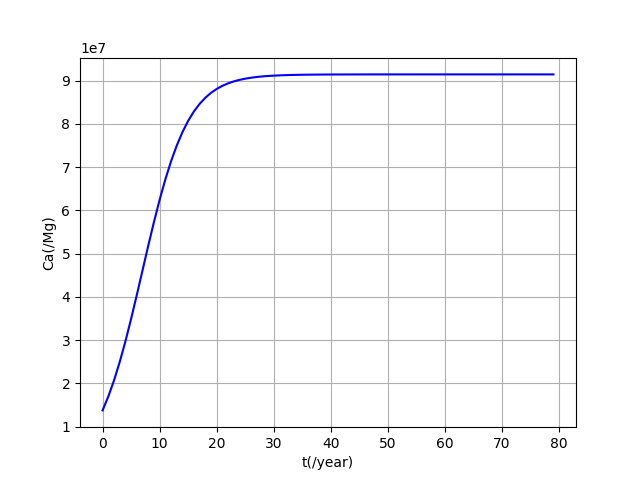
\includegraphics[width=8cm]{Ca.png}
        \caption{Image of $C_a$}
        \label{imC_a}
    \end{minipage}
    \qquad
    \begin{minipage}{8cm}
        \centering
        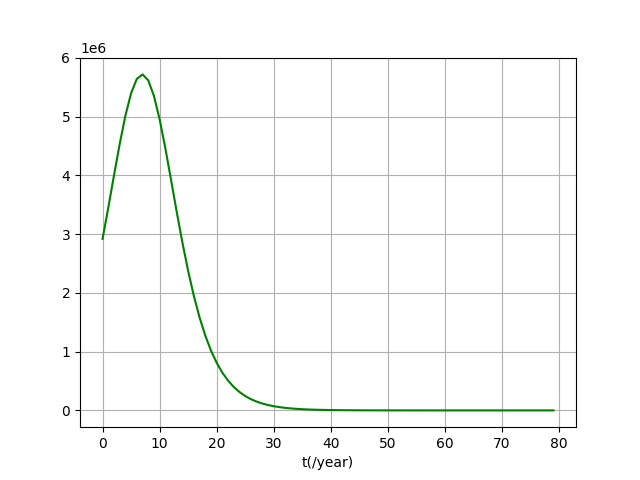
\includegraphics[width=8cm]{Ca2.png}
        \caption{Image of $C_a'$}
        \label{imC_a'}
    \end{minipage}
\end{figure}

From the function figure, we can get: Fir forests cannot grow infinitely. After
about 25 years, the fir forest reaches the limit allowed by the environmental
carrying capacity. During this process, the carbon sequestration rate first
increases and then slowly returns to zero.

To keep this forest at its maximum carbon sequestration rate, the model
recommends that deforestation begin gradually after about 7 years. According to
the model, the rate at which the loggers cut down the forest should be
consistent with the growth rate of the forest. The value of it is given by
Function \ref{speed}.
\subsection{Conclusion}
Under the premise of maximizing carbon sequestration efficiency, the forest
size should be kept at half of the maximum capacity allowed by the environment.
The felled trees will be turned into forest products, and the carbon in them
will be preserved longer. The graph of carbon content in the forest is shown in
Figure \ref{05Ca}. Forest carbon sequestration rate is shown in Figure
\ref{05Ca'}.

\begin{figure}[hp!]
    \centering
    \begin{minipage}{8cm}
        \centering
        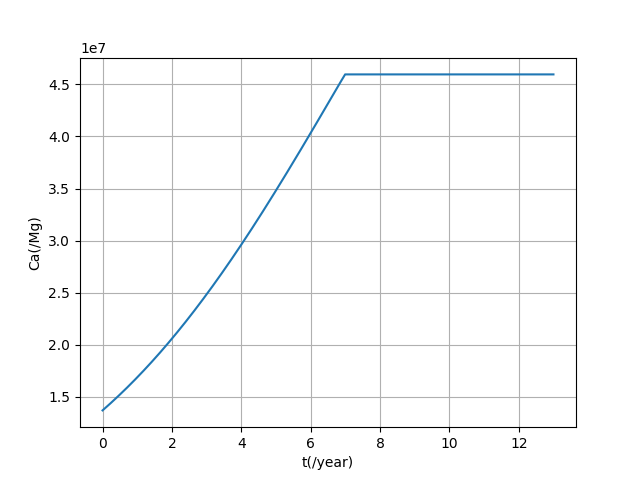
\includegraphics[width=8cm]{05Ca.png}
        \caption{Carbon Content}\label{05Ca}
    \end{minipage}
    \qquad
    \begin{minipage}{8cm}
        \centering
        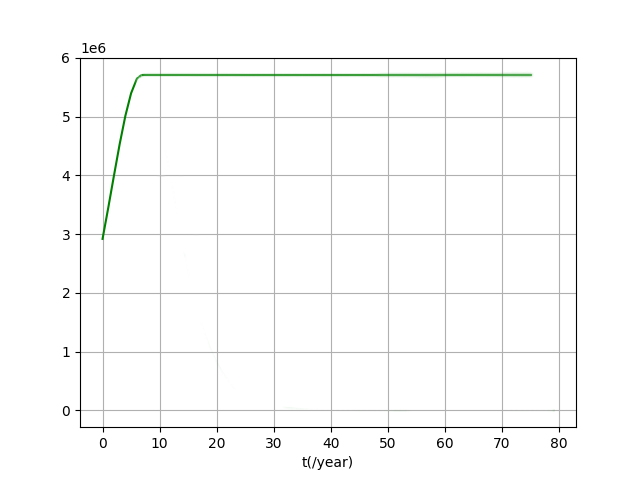
\includegraphics[width=8cm]{05Ca2.png}
        \caption{Carbon Sequestration Rate}\label{05Ca'}
    \end{minipage}
\end{figure}
The comparison between the carbon sequestration of this scheme and the forest carbon sequestration under natural growth is shown in the Figure \ref{025}.
\begin{figure}[hp!]
    \centering
    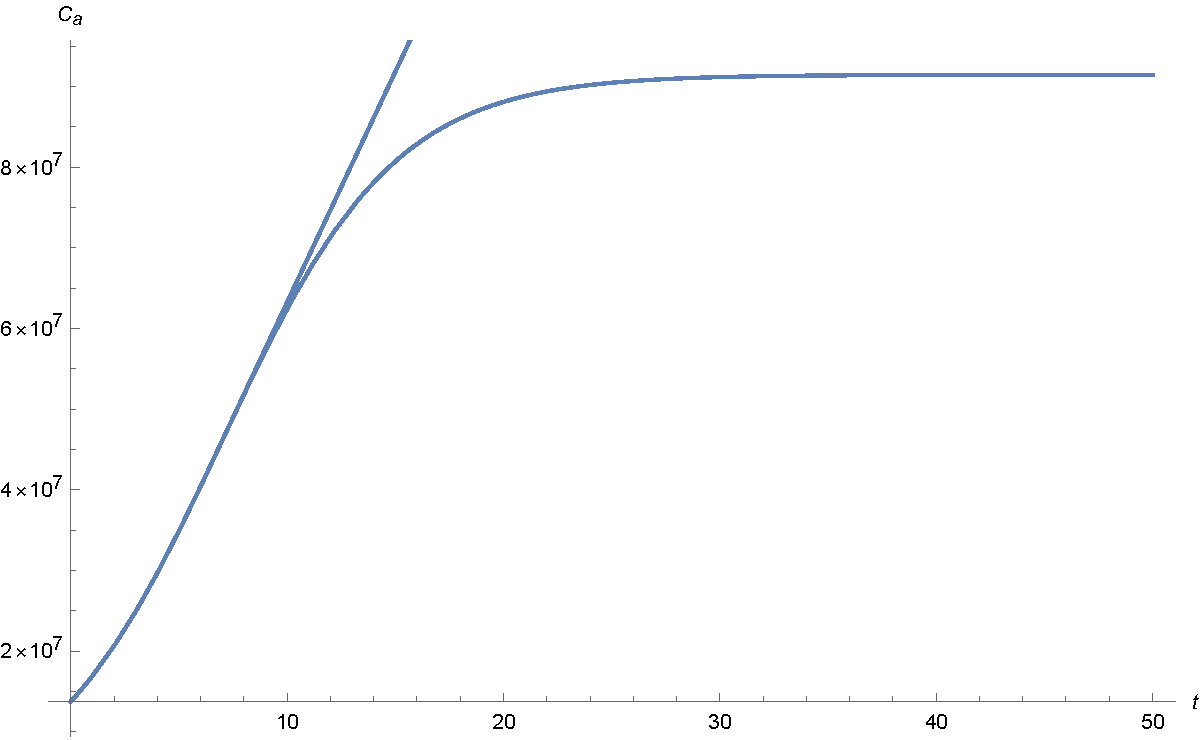
\includegraphics[width=8cm]{025.pdf}
    \caption{Carbon sequestration in forests and their products}
    \label{025}
\end{figure}

\section{Model II. Maximizing Economic Benefit Based on Logistic Growth Model}
The forest management plan that is best for carbon sequestration is not
necessarily the one that is best for society given the other ways that forests
are valued. The following model will ensure that the Forest Manager gets the
\emph{maximum benefit}.
\begin{figure}[htb]
    \centering
    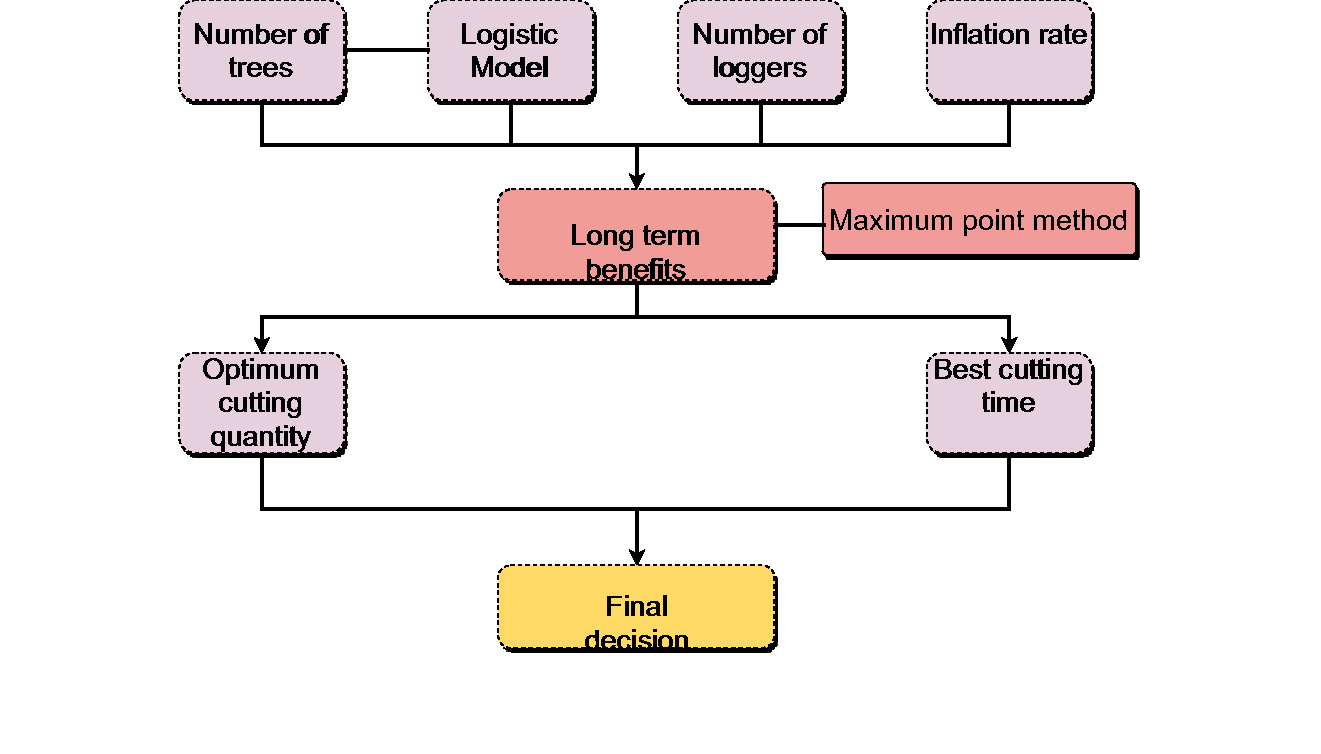
\includegraphics[width=18cm]{Model II.pdf}
    \caption{Mind map of Model II}
\end{figure}
\subsection{Model Building}
It is assumed that the natural growth of the number of trees $x(t)$ in the
forest follows the logistic law, and the amount of felling per unit time is
directly proportional to the number of loggers $u(t)$ and the number of trees
$x(t)$, which meets the following requirements:
\begin{align}
    x'(t)=  & f(x)-h(u,x)         \\
    f(x)=   & rx(1-\frac{x}{x_m}) \\
    h(u,x)= & qu(t)x(t)
\end{align}
$q$ is the cutting volume per unit time of each lumberjack.\\
Number of trees at initial time:
\begin{equation}
    x(0)=\frac{x_m}{k},k\gg1 \label{m4}
\end{equation}
$x(0)$ is very small, at time $0 \leqslant t \leqslant \tau$ no felling in it.
When $t>\tau$, the number of post fellers remains constant $U$, i.e.:
\begin{align}
    u(t)=\left\{
    \begin{array}{l@{,}l}
        0 & 0\leqslant t\leqslant \tau \\
        U & t > \tau
    \end{array}
    \right.
    \label{m5}
\end{align}
$\tau, U$ is the undetermined parameter. $x(t)$ remains stable when $t > \tau$.

The selling unit price of timber is $p$, the unit time cost of each lumberjack
is $c$, and the inflation rate (discount factor) is $\delta$. Under this
assumption, the profit per unit time is: $e^{-\delta t}$.\\ The objective
function should be the long-term benefit with $u(t)$ as the control function,
as follows:
\begin{align}
    J[u(t)] & =\int_0^\infty e^{-\delta t}[ph(u(t),x(t))-cu(t)]dt \notag \\
            & =\int_0^\infty e^{-\delta t}[pqx(t)-c]u(t)dt \label{m6}    \\
    x'(t)   & =rx(1-\frac{x}{x_m})-qu(t)x \label{m7}
\end{align}
When $0 \leqslant t \leqslant \tau$,
$x(t)$ can be solved by (\ref{m7}) under condition (\ref{m4}).\\
When $t > \tau$, $u(t)=U$, let $x'(t) = 0$. Combined with (\ref{m7}),
the constant $x(t)$ can be solved, as following:
\begin{align}
    x(t)=\left\{
    \begin{array}{l@{,}l}
        \dfrac{x_m}{1+(k-1)e^{-rt}} & 0\leqslant t \leqslant \tau \\
        x_m(1-\dfrac{qU}{r})        & t>\tau
    \end{array}
    \right.
    \label{m8}
\end{align}
$x(t)$ in $t=\tau$ is continuous, i.e.:
\begin{equation}
    \tau = \frac{1}{r}\ln [(k-1)(\frac{r}{qU}-1)] \label{m9}
\end{equation}
$\tau$, Only one quantity in U is independent. As U is independent,
Only one quantity in $\tau$ and $U$ is independent. Taking $U$ to be independent,
then $\tau=\tau(U)$, combined with (\ref{m5})(\ref{m6})(\ref{m8}), there have:
\begin{align}
    F(U) & = \int^\infty_0 Ue^{-\tau t}[pqx_m(1-\frac{qU}{r})-c]dt \notag          \\
         & = \frac{pqx_mU}{\delta}e^{-\delta\tau(U)}(1-\frac{qU}{r}-b) \label{m10} \\
    b    & = \frac{c}{pqx_m} \notag
\end{align}
It is observed that $x_m$ is the maximum number of trees,
and $b$ is the lower bound of the cost price ratio.
Obviously, $b < 1$, otherwise the cost is higher than the selling price.
From (\ref{m10}), it can be seen that the condition of benefit $F(U) > 0$ is $\frac{1-qU}{r-b}>0$,
i.e.:
\begin{equation}
    0<U<\frac{r(1-b)}{q} \label{m11}
\end{equation}
By different methods, the maximum value point of $F(U)$ under the condition of (\ref{m11}) is:
\begin{equation}
    U^*=\frac{r}{4q}\left[3-b+\frac{\delta}{r}-\sqrt{(1+b-\frac{\delta}{r})^2+\frac{8b\delta}{r}}\right]
    \label{m12}
\end{equation}
Combined with (\ref{m9})(\ref{m12}), $\tau^*=\tau(U^*)$.\\
So the $U^*$ and $\tau^*$ are the best number and time for felling.

\subsection{Difference between Model I and Model II}
Typically, inflation is very low. To facilitate the analysis of horses, here we
set $\delta$ to 0. At this time, Equation (\ref{m12}) is simplified to the
following form:
\begin{equation}
    U_0=\frac{r}{2q}(1-b) \label{A1}
\end{equation}
Plug $U_0$ into Equation (\ref{m8}), we get the following data:
\begin{equation}
    x(t)=\frac{c}{2pq}+\frac{x_m}{2},(when:t>\tau,Steady\ state\ value)
\end{equation}
\begin{figure}[htb]
    \centering
    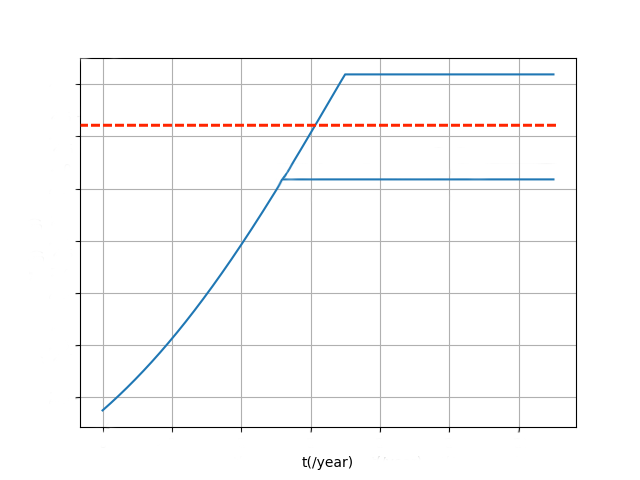
\includegraphics[width=10cm]{compare.png}
    \caption{Comparison of Forest Size in Model I and Model II}
\end{figure}
This is the steady-state value of forest size after deforestation begins.
Compared with Model I
\[x(t_m)=\frac{x_m}{2}\]
This value increases a part of the coefficient.We call it the economic impact
factor and denote it as $B$.
\[B=\frac{c}{2pq}\]

The economic impact factor($B$) and the cost-to-price ratio($b$) together
determinethe forest manager's management strategy for the forest, that is, the
size of the forest to be controlled.

For different forests: affected by factors such as forest location, forest
climate, and local economic development level, the final steady-state size of
the forest will change to varying degrees. However, in order to balance the
carbon sequestration rate and economic benefits, the final steady-state size of
the forest should be kept between
\[\frac{x_m}{2}\]
and
\[\frac{c}{2pq}+\frac{x_m}{2}\]

According to the model analysis, under normal circumstances, the forest must be
cut down. If and only if the forest management agency is incapable of managing
the forest, it may lead to the forest not being cut down.

\subsection{Felled or Not}
As mentioned above, we know the amount and timing of deforestation. Now let’s
discuss what kind of tree is felled under the conditions of time $\tau$. It is
considered that the following two situations occur in the felled trees:
\begin{enumerate}
    \item The trees are in poor health. If they are not cut down, the trees will absorb
          nutrients and affect the growth of other trees.\label{e1}%%
    \item Trees already have high economic value.\label{e2}
\end{enumerate}

Firstly, let's discuss point \ref{e1}. Assuming that the health of trees is
related to time $t$ and environmental condition $x$, i.e.: $f(t,x)$. It is
considered that $x=0$ represents that the environment has no impact on the
trees, and $f(0,0)=1$ represents that the trees are in a completely healthy
state. When $f(t,x)=0$, it is considered that the trees are completely dead. We
find that $f(t,0)$ is only related to time or age. According to common sense,
the image of $f(t,0)$ is roughly as follows(Figure \ref{F1}):
\begin{figure}[htb]
    \centering
    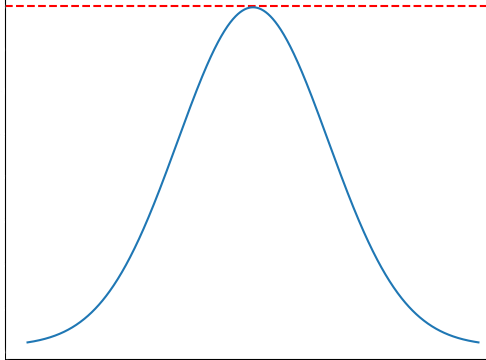
\includegraphics[width=8cm]{ftx.png}
    \caption{$f(x,t)$}\label{F1}
\end{figure}
Assuming that $t$ and $x$ of all trees in a forest are known,
when $f (t, x) \leqslant 0.1$, the trees are no longer suitable for survival and must be cut down.
There are $N$ trees in total, and $n$ trees are conforming to the above formula.
It can be seen from the above that $qU^*$ trees need to be cut down at this time.

If $n \geqslant qU^*$, trees with a smaller $f$ value will be cut first. If $n
    \leqslant qU^*$, $qU^*-n$ trees will still be cut down. Then discuss \ref{e2}.
As mentioned above, the selling unit price of wood is $p$, we assume that $p$
is fluctuating, and we think that $p$ is related to the timber volume $V$ of
trees. That is, $p(V)$, and the functional relationship that $p(V)$ should meet
is roughly as follows: (Figure \ref{F2})
\begin{figure}[htb]
    \centering
    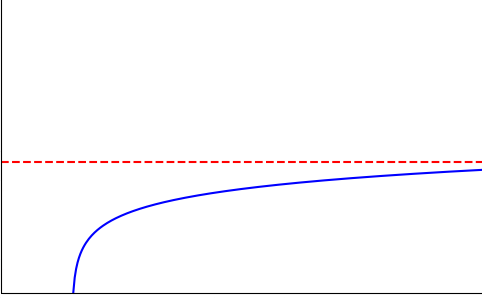
\includegraphics[width=8cm]{pV.png}
    \caption{$p(v)$}\label{F2}
\end{figure}\\

Note: if the volume of trees is too small, it is obvious that no merchant is
willing to buy them; No matter how large the volume of a single tree is, its
selling unit price must have a threshold.

In this way, we can select $qU^* - n$ trees with large $p(V)$ value among $N-n$
trees.

\section{Transition Points between Management Plans}
In the above two decision-making plans and the "balanced plans", there are only
two management plans:
\begin{enumerate}
    \item Conservation and cultivation: Make the forest develop rapidly.
    \item Maintaining the size of forest stable(ie: cutting down at the rate of forest
          growth).
\end{enumerate}
According to the analysis process above,
the \emph{Transition Points} of these two management plans is when the forest size reaches the desired state.
Such as:$\dfrac{x_m}{2}$ or $\dfrac{c}{2pq}+\dfrac{x_m}{2}$.

In addition, we provide a brand new thinking direction (Inheriting the idea of
Model II):

Start timing from 0, and set the original time $t_0$. \\ It can be seen from
the above that the best time to cut down is $\tau^*$. Now we discuss the
felling time. The felling time of a single tree by a woodcutter should be
directly proportional to the strength of the number and inversely proportional
to the physical strength of the woodcutter. The physical strength of the
woodcutter decreases with time. When the woodcutter has sufficient physical
strength, the workload per unit time is large and the physical strength
decreases rapidly, so the image of the woodcutter's physical strength function
is roughly as Figure \ref{602}.
\begin{figure}[ht]
    \centering
    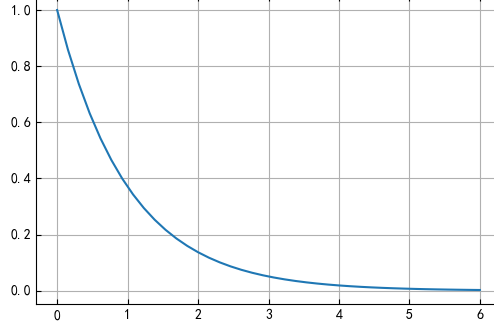
\includegraphics[width=9cm]{602.png}
    \caption{Woodcutter's Physical Strength}
    \label{602}
\end{figure}\\
Our simulation is:
\[g(t)=e^{-at}\]
$a$ is related to personal health status. Assuming that the average strength of trees is $b$
and $b$ remains unchanged during logging if the time spent by loggers cutting a single tree is
negligible compared with the whole logging project when the loggers start a certain logging
function at time $t$:
\[T(t)=k\frac{b}{e^{-at}}\]
Then there are:
\[T(0)=kb=t_1,\ T(kb)=\frac{kb}{e^{-akb}}=t_2,\ T(t_2)=t_3\dots\]
Total time:
\[T=t_1+t_2+t_3+\dots\]
Assuming that each woodcutter cuts down $d$ trees, there are:
\[T=t_1+t_2+t_3+\dots+t_d\ d=t_{d-1},\ \tau^*+T=t_0+10\]
Therefore, the scheme we give is that the economic investment in this forest
needs to be increased to the original scheme $\dfrac{\tau^*+T}{t_0}$ times. The
reason for it is that the new scheme may have small fluctuations due to
uncertain factors.
\subsection{Examples of Forest Management Plans}
\subsubsection{Carbon dioxide absorption in 100 years} \label{611}
Here, we still use the data from \emph{Analysis of Model I}
%	According to Equation \ref{C_a'}, the time to felling the forest is $t=6.933 years$.
%	After this time, the rate of forest carbon sequestration is about $5.71680\times 10^6Mg/y$.\\
%	So after 100 years, the carbon sequestration of forests and their products is $5.77776\times 10^8 Mg$.
Bringing the data into Function (\ref{C_a}), we get:
\begin{align}
    C_a = & Y_b/2=\frac{a S V_a x_m}{2\left(\frac{x_m}{x_0}-1\right) e^{-r t}+2}+\frac{b}{2} \notag \\
    =     & 11.2705\, +\frac{1.82938\times 10^8}{11.32 e^{-0.25 t}+2} \label{6.1}
\end{align}
Derive Function (\ref{6.1}):
\begin{equation*}
    C_a'=\frac{5.17714\times 10^8 e^{-0.25 t}}{\left(11.32 e^{-0.25 t}+2\right)^2}
\end{equation*}
The extreme point of this function is:
\begin{align}
                & \text{Maximize}\left[\frac{5.17714\times 10^8 e^{-0.25 t}}{\left(11.32 e^{-0.25 t}+2\right)^2},\{t\}\right] \notag \\
    \Rightarrow & \notag                                                                                                             \\
                & \{5.7168\times 10^6,\{t\to 6.9337\}\} \notag
\end{align}
Therefore, when $t$ is $6.93$ (i.e.:6.93 years), the carbon sequestration rate reaches the maximum.
Deforestation at this time (keeping the forest size unchanged), the forest carbon sequestration rate will always remain at the maximum rate.
At this time, the forest has sequestered carbon of $4.57133\times 10^7$.

After that, using a typical linear prediction model, the prediction function
is:
\[\hat{C}_a=5.7168\times 10^6 (t-6.93)+4.57133\times 10^7(Mg)\]
Thus, after 100 years, the amount of carbon sequestered by forests and their
products is $5.77776\times 10^8Mg$
\subsubsection{Selection of Forest Management Plan}
The specific choice of forest management scheme is closely related to local
economic conditions. If the local economy is dominated by forests, the forest
management plan is more inclined to Model II; if the local economic development
has nothing to do with forests, we recommend the Model I plan.

According to the situation of this forest, the forest management plan of
protection and cultivation should be adopted in the current situation. Because
the current forest size has not reached the scale corresponding to the maximum
carbon sequestration rate. After about 7 years, the forest scale has reached
the corresponding maximum carbon sequestration rate. At this time, some
overripe and mature trees should be cut down according to the felling principle
in order to maintain the maximum carbon sequestration rate.
\begin{table}[htb!]
    \centering
    \begin{tabular}{c>{\centering\arraybackslash}p{14cm}}
        \toprule
        \textbf{Time(year)} & \textbf{Forest Management}                                                        \\
        \midrule
        $t<6.93$            & Conservation and Cultivation                                                      \\
        \midrule
        $t>6.93$            & Deforestation at the same rate as forest growth, in order to maintain forest size \\
        \bottomrule
    \end{tabular}
\end{table}

\section{Model Evaluation}
\subsection{Strengths}
\begin{itemize}
    \item There are many factors affecting plantation growth, but all populations fit the
          Logistic Growth Model when well managed. Both Model I and Model II are plans
          made directly based on the Logistic Growth Model and have high reliability.  %%
    \item In Model II, we comprehensively consider various factors including inflation
          rate ($\delta$), lumberjack wages($c$), and the market price of lumber($p$).
          Model coverage is comprehensive. %
\end{itemize}
\subsection{Weaknesses}
\begin{itemize}
    \item For natural forests, the variables required for prediction are difficult to
          measure directly.
\end{itemize}

\section{Conclusion}
\begin{enumerate}
    \item We predicted the forest growth law through the Logistic Growth Model, and
          calculated the actual carbon sequestration and carbon sequestration rate of the
          forest in combination with the BEF. %
    \item Through differential equations, we obtain the logging scale and the number of
          loggers on the premise of ensuring the best economic benefits. %
    \item By comparing Model I with Model I, we developed a concrete plan for determining
          forest size.
    \item By analysing trees at different growth stages, we derive specific felling
          strategies
    \item We use the above two models to predict the amount of forest carbon
          sequestration in 100 years.
\end{enumerate}

%%%%%%%%%%%%%%%%%%%%%%%%%%%%%%%%%%%%%%%%%%%%%%%%%%
%\newpage
%\section*{The Forest Said: I Can't Eat Anymore! \textsl{---Newspaper Article}}
\twocolumn[\section*{\texttt{The Forest Said: I Can't Eat Anymore!}\\  \raggedleft\textsl{---Newspaper Article}}]
\addcontentsline{toc}{section}{\texttt{The Forest Said: I Can't Eat Anymore!} \textsl{---Newspaper Article}}

The traditional view is that we can never cut down trees for any reason. Our
research found that this is not the case. No matter what kind of trees, no
matter how they grow, they will age or even die. It is undeniable that the
greatest function, or purpose, of planting trees is to protect the environment,
such as wind prevention, sand fixation, air purification, and so on. Our
research shows that when a tree reaches a certain age, its direct value will be
greatly reduced. In addition, it will continue to absorb nutrients from the
soil. In this way, it will affect the growth of other trees. Although from a
scientific point of view, nutrients will be returned to the soil after the tree
dies, and there is not much loss of nutrients in general, But we think this
process is too long, especially for tall trees, which requires a lot of
decomposers to work for a long cycle. In other words, in this process, the
residual value of the tree has not been fully utilized. Although it has no
great impact on the overall environment, we always hope for better results. If
we can make better use of the economic value of the tree, more funds will be
invested in the construction of the local ecological environment. We think this
process is beneficial to the tree population from the perspective of results.
Firstly, the carbon sequestration we are most concerned about has only a small
reduction in this process, which is completely negligible from a mathematical
point of view. Cutting down trees does not affect the most important carbon
sequestration function of the tree population. Secondly, we can provide a
rigorous and reasonable forest management plan and analyze the most reasonable
cutting quantity and cutting time with data, We can even elaborate on which
trees are retained and which trees are cut down. Finally, we can put forward
efficient forest regeneration schemes to protect the environment of the local
government to the greatest extent. In general, we believe that logging should
not be prohibited. At least in terms of forest management, appropriate and
planned logging can bring more benefits to forests.

The comparison between mature trees and over mature trees is shown in the
figure below:
\begin{figure}[ht]
    \centering
    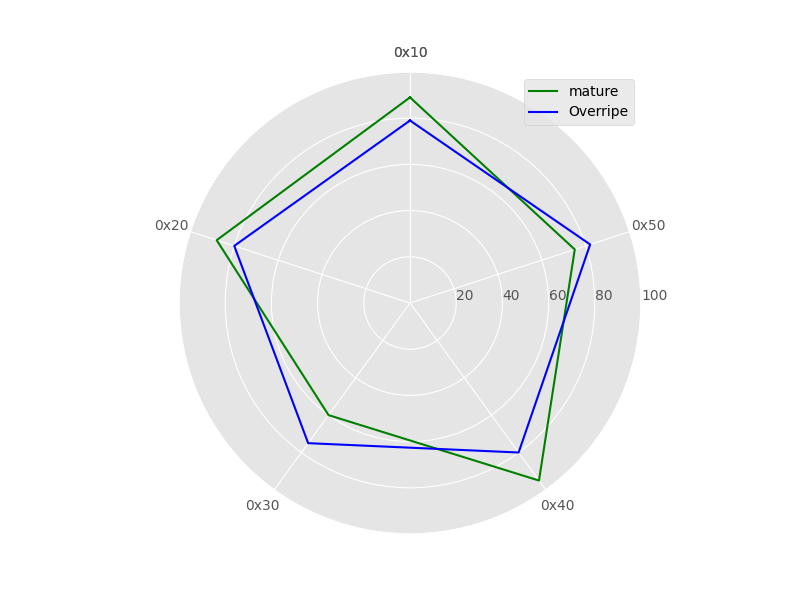
\includegraphics[width=9cm]{News1.png}\\
    (Where 0x10 represents the carbon fixation capacity, 0x20 represents the wind and sand fixation capacity, 0x30 represents the occupation of natural resources, 0x40 represents the economic value, and 0x50 represents the maintenance consumption fund.)
\end{figure}
\onecolumn
%%%%%%%%%%%%%%%%%%%%%%%%%%%%%%

%%%%%%%%%%参考文献
\newpage
\printbibliography %%%参考文献数据库,使用\cite{bibid}在需要的地方引用参考文献
\addcontentsline{toc}{section}{\textit{References}}
\newpage
%%%%%%%%%附录区域
\appendix
\section{Program Source Code}
\subsection{Python Code for Figure \ref{imC_a}}
\begin{python}
    import numpy as np
    import matplotlib.pyplot as plt
    x=np.arange(0,80,1)
    y=0.3999*1e7*137.375*0.333/(2*(0.333/0.05-1)*np.exp(-0.25*x)+2)+11.27
    plt.figure()
    #plt.style.use('ggplot')
    plt.plot(x,y,linestyle='-',color='blue')
    plt.xlabel('t(/year)')
    plt.ylabel('Ca(/Mg)')
    plt.grid()
    plt.show()
\end{python}
\subsection{Python Code for Figure \ref{imC_a'}}
\begin{python}
    import numpy as np
    import matplotlib.pyplot as plt
    x=np.arange(0,80,1)
    y=2*0.3999*0.25*1e7*137.375*0.333*(0.333/0.05-1)*np.exp(-0.25*x)/(2*(0.333/0.05-1)*np.exp(-0.25*x)+2)/(2*(0.333/0.05-1)*np.exp(-0.25*x)+2)
    plt.figure()
    plt.xlabel('t(/year)')
    plt.plot(x,y,linestyle='-',color='green')
    plt.grid()
    plt.show()
\end{python}
\section{Parameters used to calculate biomass expansion factor (BEF)}
\centering
\begin{tabular}{>{\centering\arraybackslash}p{8cm}cc*{2}{>{\centering\arraybackslash}p{1.5cm}}}
    \toprule
    \textbf{Forest type}                   & $a(Mg/m^3)$ & $b(Mg)$ & $N$ & $R^2$ \\
    \midrule
    Abies and Picea                        & 0.4642      & 47.4990 & 13  & 0.98  \\
    Betula                                 & 1.0687      & 10.2370 & 9   & 0.70  \\
    Casuarina                              & 0.7441      & 3.2377  & 10  & 0.95  \\
    \rowcolor{pink}Cunninghamia lanceolata & 0.3999      & 22.5410 & 56  & 0.95  \\
    Cypress                                & 0.6129      & 46.1451 & 11  & 0.96  \\
    Deciduous oaks                         & 1.1453      & 8.5473  & 12  & 0.98  \\
    Eucalyptus                             & 0.8873      & 4.5539  & 20  & 0.80  \\
    Larix                                  & 0.6096      & 33.8060 & 34  & 0.82  \\
    Lucidophyllous forests                 & 1.0357      & 8.0591  & 17  & 0.89  \\
    Mixed conifer and deciduous forests    & 0.8136      & 18.4660 & 10  & 0.99  \\
    Mixed deciduous andSassafras           & 0.6255      & 91.0013 & 19  & 0.86  \\
    Nonmerchantable woods                  & 0.7564      & 8.3103  & 11  & 0.98  \\
    Pinus armandii                         & 0.5856      & 18.7435 & 9   & 0.91  \\
    P. koraiensis                          & 0.5185      & 18.2200 & 17  & 0.90  \\
    P. massoniana, P. yunnanensis          & 0.5101      & 1.0451  & 12  & 0.92  \\
    P. sylvestris var. mongolica           & 1.0945      & 2.0040  & 11  & 0.98  \\
    P. tabulaefomis                        & 0.7554      & 5.0928  & 82  & 0.96  \\
    Other pines and conifer forests        & 0.5168      & 33.2378 & 16  & 0.94  \\
    Populus                                & 0.4754      & 30.6034 & 10  & 0.87  \\
    Tsuga, Cryptomeria, Keteleeria         & 0.4158      & 41.3318 & 21  & 0.89  \\
    Tropical forests                       & 0.7975      & 0.4204  & 18  & 0.87  \\
    \bottomrule
\end{tabular}
\newpage
\section{Effects of Different Growth Rates on Carbon Sequestration}
\begin{figure}[hp!]
    \centering
    \begin{minipage}{8cm}
        \centering
        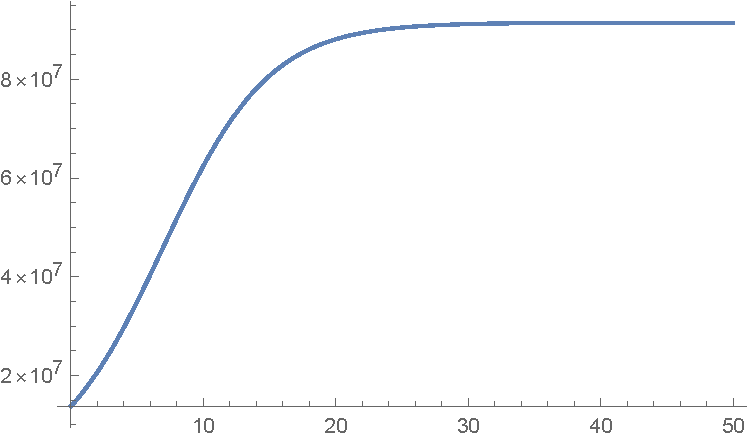
\includegraphics[width=8cm]{C025.pdf}
        \caption{$r=0.25$}
    \end{minipage}
    \qquad
    \begin{minipage}{8cm}
        \centering
        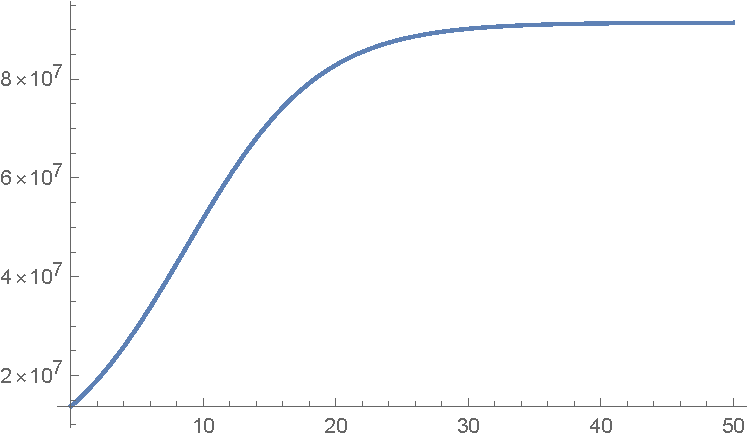
\includegraphics[width=8cm]{C020.pdf}
        \caption{$r=0.20$}
    \end{minipage}\\
    \begin{minipage}{8cm}
        \centering
        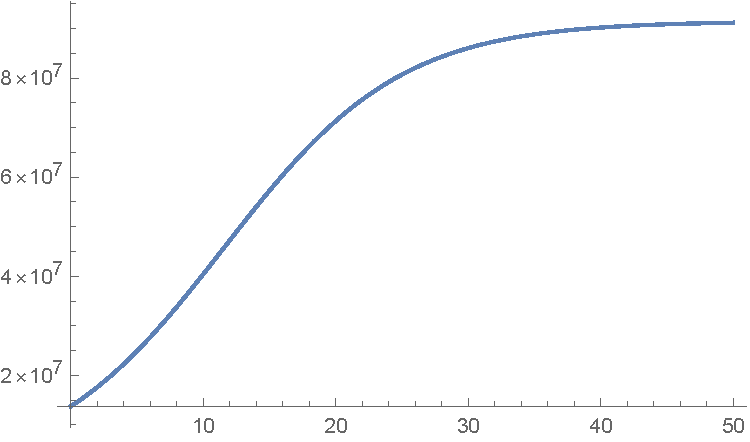
\includegraphics[width=8cm]{C015.pdf}
        \caption{$r=0.15$}
    \end{minipage}
    \qquad
    \begin{minipage}{8cm}
        \centering
        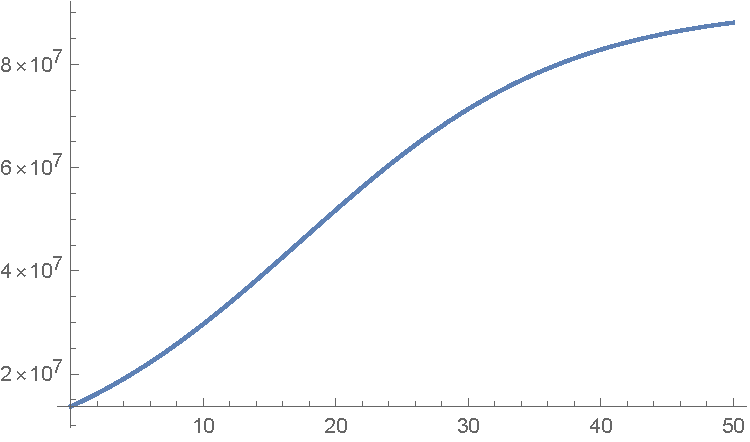
\includegraphics[width=8cm]{C010.pdf}
        \caption{$r=0.10$}
    \end{minipage}
\end{figure}
\end{document}